\documentclass{article}
\usepackage{amsmath}
\usepackage{graphicx} % Required for inserting images

\title{Exercise 1}
\author{Haim Lavi, 038712105}
\date{May 2025}

\begin{document}

\maketitle

a. We write the discrete time transition matrix:
\[
P=(p_{ij})=\begin{pmatrix}
    0 & 1 & 0 \\
    0.5 & 0 & 0.5 \\
    0 & 1 & 0 \\
\end{pmatrix}
\]
then $q_{ij}=p_{ij}\cdot\lambda_i$ and $q_{ii}=-\lambda_i$, hence
\[
Q=(q_{ij})=\begin{pmatrix}
    -1 & 1 & 0 \\
    1 & -2 & 1 \\
    0 & 3 & -3 \\
\end{pmatrix}
\]
b. We find the only solution to the equation $\pi{Q}=0$, where $\pi=\begin{pmatrix}
    \pi_1 & \pi_2 & \pi_3
\end{pmatrix}$, such that $\pi_1+\pi_2+\pi_3=1$. This gives the following system of equations:
\begin{flalign}
-\pi_1+\pi_2=0\\
\pi_1-2\pi_2+3\pi_3=0\\
\pi_2-3\pi_3=0
\end{flalign}
Hence, $\pi=\begin{pmatrix}
    3\pi_3 & 3\pi_3 & \pi_3
\end{pmatrix}=\begin{pmatrix}
    \frac{3}{7} & \frac{3}{7} & \frac{1}{7}
\end{pmatrix}$

c. There are several possible sources for an error:
\begin{enumerate}
    \item 
\end{enumerate}
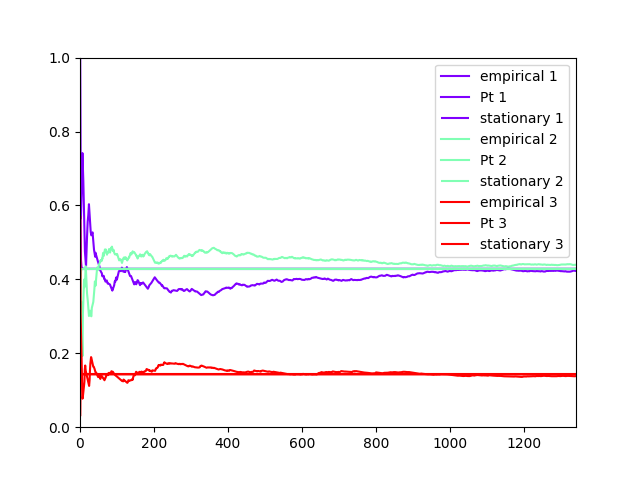
\includegraphics{ctmc1.png}
\end{document}
